
\chapter{Bifurcation theory}
\label{chap:bifurcation-theory}

Phase plane analysis helps us to analyze the behavior of a two-dimensional
system, consisting of two coupled equations (Appendix
\ref{chap:phase-plane-analysis}). In this Appendix, we study with the stability
of the fixed-points. 

\citep{rinzel1983}

\section{Stability of a system}
\label{sec:stability}

Stability means the small perturbations to the parameters, at which the system
is at equilibrium, produce a small perturbations in the solution.

More on Sect.\ref{sec:stability-near-fixed-points}.

\subsection{Fixed point}
\label{sec:fixed-point}

A fixed point is a point that does not change upon application of a map, or a function, etc. 
\begin{equation}
x_0 = f(x_0)
\end{equation}
with $f(\cdot)$ represents such a map, or a function of interested.

In time-discrete system, the solution that

\begin{equation}
  \label{eq:637}
  x(t+1) = f(x(t))
\end{equation}
is called {\bf fixed-point}.



In an ODE system, the points of an autonomous system of ordinary differential
equations at which $\mathbf{f(x)} = 0$ are also known as fixed points. Fixed
points are also called critical points or equilibrium points -
Sect.\ref{sec:equilibria}. A fixed point can be classified into one of several
classes using linear stability analysis and the resulting stability matrix.


{\bf NOTE}: 
\begin{enumerate}
\item {\bf Fixed-point}\footnote{\url{http://math.fullerton.edu/mathews/n2003/FixedPointMod.html}} is the solution of the equation $x=g(x)$. 
  Geometrically, it is the intersection of the curve $y=g(x)$ and the
  line $y=x$. 
  
\item The fixed-point values of a number of common functions are given in 
\url{http://mathworld.wolfram.com/FixedPoint.html}

Example:
\begin{verbatim}
FUNC NAME           |   FIXED-POINT

cosine                 0.7390851332


tangent                4.4934094579


\end{verbatim}

\item For a system in $\mathbb{R}^n$ space, then any
  lower-dimensional space is called the {\bf Poincar\'e section} S. 

\item When a Poincar\'e section intersect with the periodic orbit of
  the system at the point $x$, consider a function $P$ that map every
  point $\sigma$ on S that is in an appropriate neighborhood to $x$ to
  a point on the Poincar\'e section, i.e. $P(\sigma)$. If the
  projected 
  point $P(\sigma)$ is also the starting point $\sigma$ also,
  i.e. $\sigma=P(\sigma)$, 
  then $P$ is known as
  the 
  {\bf Poincar\'e map} for the orbit, as shown in
  Fig.~\ref{fig:Poincare_map}\footnote{\url{http://en.wikipedia.org/wiki/Poincaré_map}}. 

\begin{figure}[hbt]
  \centerline{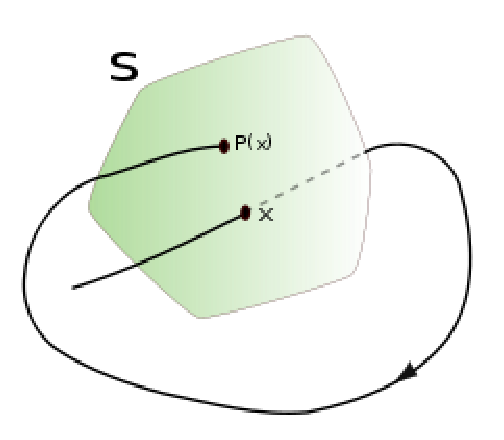
\includegraphics[height=4cm,
    angle=0]{./images/Poincare_map.eps}}
\caption{S is the Poincar\'e section, the Poincar\'e map (or first
  recurrence map) P projects point x onto P(x)}
\label{fig:Poincare_map}
\end{figure}


\item As the system is periodic with $x_\tau$, if $\sigma=x$, then
  $P(x)=x$ or $x$ the fixed-point of the system.

\end{enumerate}

In our case, if $(\mu_0,x_0)$ is the fixed-point, we can also move it
to the origin by a change in coordinates
$x=x-x_0,\mu=\mu-\mu_0$. Thus, without losing the generality, we can
assume that the system's fixed point is at the origin $(0,0)$.

Consider a discrete-time non-linear system with periodic cycle
$\tau$. Then $x_\tau(t) = x_\tau(t+\tau)$.


\subsection{Equilibria (fixed-points)}
\label{sec:equilibria}

For a time-continuous system represented by a set of ODE,
\begin{equation}
  \label{eq:636}
  \dot{x}=f(x)
\end{equation}
the {\bf equilibria} points are the point on the nullclines,
i.e. $f(x)=0$. They are time-independent solution of the system.
\begin{equation}
\begin{split}
\frac{dx_1}{dt} = f_1 (x_1, x_2, \ldots, x_n) = 0 \\
\ldots \\
\frac{dx_n}{dt} = f_n (x_1, x_2, \ldots, x_n) = 0 \\
\end{split}
\end{equation}


In an ODE system, the points of an autonomous system of ordinary differential
equations at which $\mathbf{f(x)} = 0$ are also known as fixed points -
Sect.\ref{sec:fixed-point}. So, equilibrium points and fixed-points are the same.

\subsection{critical point}
\label{sec:critical-point}

A function $y=f(x)$ has critical point $x_0$ where 
\begin{itemize}
  \item  $f'(x_0) = 0$
  
  \item or $f(x)$ is not differentiable
\end{itemize}


A function $z=f(x,y)$ has critical points $(x_0, y_0)$ where

\begin{itemize}
  \item  the gradient $\nabla f = 0	$
  
  \item the partial derivative $\partial f/ \partial x$ is not defined.
\end{itemize}

\subsection{Behavior of a system near fixed-points}
\label{sec:stability-near-fixed-points}

If a system is in equilirbium, and then its variable is slightly
displaced from a fixed point, the system can behave in one of the following ways

\begin{enumerate}
  \item  (1) move back to the fixed point ("asymptotically stable" or "superstable"), 
  
  
  \item (2) move away ("unstable"), or 
  
  \item (3) move in a neighborhood of the fixed point but not approach it
  ("stable" but not "asymptotically stable").
  
\end{enumerate}

Because of this, fixed points are also called critical points
(Sect.\ref{sec:critical-point}) as it helps us to understand the behavior of a
system of interest.

In order to analize a behaviour of solutions near fixed points, the below techniques can be used
\begin{enumerate}	
  
  \item linearization of the system (Sect.\ref{sec:linear-appr-non-linear}) into
  $\dot{x} = A.x$
  
  \item then, stability of a fixed point can be determined by eigen values of matrix 
  
NOTE: the matrix $\mathbf{A}$ if it has eigenvector $v$ and eigenvalue $\lambda$
(Sect.\ref{sec:eigenvalues-method}), then we know that the solution of the
aboved linearized system is of the form
\begin{equation}
x = e^{\lambda t} v
\end{equation}
\end{enumerate}w


\subsection{-- Stable fixed-point (as in Hopf birfucation)}
\label{sec:stable-equilibria}

An equilibrium point (or fixed-point), of a system represented by the set of
ODEs, is stable if the system, start from a point near the equilibrium point,
will stay near the equilibrium point, i.e. never get back to the exact
equilibrium point.

Suppose a system $\dot{x}=f(x)$ with equilibrium point $x_e$.
Mathematically, we can say that given any distance $R$, there exist a
distance $r$ such that there exist a point $f(0)$ near $x_e$,
i.e. $|f(0)-x_e<r$, and the trajectory of the system is always close
to $x_e$, i.e. $|f(t)-x_e|<R$, for all $t\ge 0$.

When the system is disturbed causing the loss in stability, and the system form
a {\bf closed orbit} around $x_e$ (an oscillation), we call it {\bf Hopf
bifurcation} (Sect.\ref{sec:hopf-bifurcation}). 

The local stability is examined by linearization of the dynamics at the
intersection (the fixed-point) (Sect.\ref{sec:linear-appr-non-linear}).
\begin{equation}
\frac{d}{dt}\vect{x} = \left( \begin{array}{cc} 
F_u & F_w \\
G_u & G_w 
\end{array}\right) \vect{x}
\end{equation}

\textcolor{red}{Stability of the fixed-point requires the real part of both
eigenvalues be negative}. The necessary and sufficient condition for stability
is 
\begin{equation}
F_u + G_w < 0 ; F_uG_w - F_wG_u > 0
\end{equation}

If $F_uG_w - F_wG_u < 0$, i.e. the imaginary part of both eigenvalues vanished.
Then, if one eigenvalue is positive and the other one is negative; the
fixed-point is the saddle point, see Sect.\ref{sec:eigenvalues-method}.


\subsection{-- Asymptotically stable fixed-point}
\label{sec:asympt-stable}

An asymptotically stable equilibria if it is {\bf stable equilibria} (Sect.\ref{sec:stab-equil}),
and in addition, for the small perturbation in the control parameter,
the state of the system converge to equilibrium state as the time
increases\footnote{\url{http://www.cds.caltech.edu/~murray/amwiki/Dynamic_Behavior}}.
The second criteria is known as the
{\it attractivity of the equilibrium point}.

Mathematically, the addition condition is that
\begin{equation}
  \label{eq:655}
  \lim_{t\rightarrow \infty} |f(t)-x_e| = 0
\end{equation}

Consider $x_e$ is the equilibria point of the system,
i.e. $V(\mu,x_e)=0$. Then the original system is said to be
{\bf asymptotically stable} at the equilibrium if all eigenvalues have
negative real parts $Re(\lambda)<0$. The original system is unstable
at this equilibrium if at least one eigenvalue has positive real part.

% This criteria is important as when we can prove $x_e=0$ is
% asymptotically stable 
\subsection{Hyperbolic equilibria}
\label{sec:hyperb-equil}

The system is said to be {\bf hyperbolic equilibria} if all
eigenvalues have non-zero real parts. Hyperbolic equilibria system are
{\it robust} at that equilibrium point, i.e. it doesn't change
qualitatively the phase portrait of the system for a small
disturbance.

If there is at least one eigenvalue with zero real part, or the
eigenvalue is zero, then the system is said to be {\bf
  non-hyperbolic}, and non-hyperbolic equilibria are non-robust. A
small disturbance thus can cause local bifurcation.

\url{http://www.scholarpedia.org/article/Equilibria}.

\section{Introduction}
\label{sec:introduction-3}

The concept of bifurcation theory started with Euler's classical work
(1744). However, the modern development of the work starts with
Pointcar\'e and qualitative theory of differential equations. 

Instead of answering the quantitative question ``what/when/...'',
bifurcation theory is a qualitative field that answer the question
``whether/if...''.  The field of bifurcation theory deal with
dynamical {\it non-linear} systems. Such systems can be
time-continuous or time-discrete, and are often modelled in the form
of differential equations (PDE/ODE) or {\bf iterative maps},
respectively.
\begin{itemize}
\item iterated map: $x_{n+1}=f(x_n)$
\item differential equation: $\frac{dx}{dt} = f(x)$
\end{itemize}
Then, bifurcation studies how the general behavior (i.e. the solution)
of the system change when its parameters vary. Any large scale change
is called a {\bf bifurcation} and the value of the parameters at which
the change occur is called {\bf bifurcation point}. The large scale
change can be
\begin{itemize}
\item the system loose its stability
\item the appearance/disappearance of equilibria, periodic points, or
  strange attractors
\end{itemize}
Normally, bifurcation is studied at equilibria of a non-linear system
(read Sect.~\ref{sec:equilibria}), and focusing on local
stability. So, all bifurcations, by default, are for local stability. 

By qualitative studying, we can avoid plotting a phase portrait with
multiple trajectories like the one shown in
Fig.~\ref{fig:phase_curve}, yet still can have a geometrical view of
the topological change of the system without drawing all phase curves.

% When multiple phase curves corresponding to different initial
% conditions are plotted in the same phase plane, the result is known as
% {\bf phase portrait}.

\begin{figure}[htb]
  \centerline{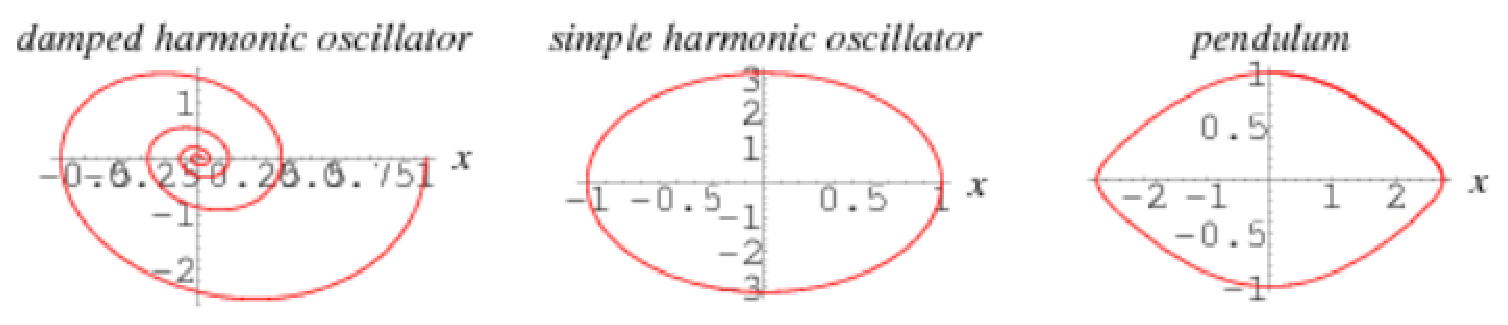
\includegraphics[height=2.3cm]{./images/phase_curve.eps}}
  \caption{Phase curves (phase flows) of some simple
    systems}\label{fig:phase_curve}
\end{figure}


Before studying the bifurcation of a system, we need a uniform way to
represent the system. In the previous chapter, we've learnt that any
non-linear system of any order can be converted to a system of
homogeneous first-order ODEs (read Sect.~\ref{sec:linear-system}).

{\bf Example}: For a system of continuous time
\begin{equation}
  \label{eq:576}
  \ddot{y} + \dot{y} + y + y^3 = 0
\end{equation}
is converted to
\begin{equation}
  \label{eq:631}
  \frac{d}{dt}\left[
    \begin{array}{c}
      x_1 \\ x_2
    \end{array} \right]
 = \left[
   \begin{array}{c}
     x_2 \\
     -x_2 - x_1 - x_1^3
   \end{array}
\right]
\end{equation}
with $x_1=y, x_2=\dot{y}$. A compact form of the system in first-order
ODE is the {\bf vector field} form
\begin{equation}
  \label{eq:632}
  \mathbf{\dot{x}} = V(\mu, \mathbf{x})
\end{equation}
with $\mu\in \mathbb{R}$, $\mathbf{x}\in \mathbb{R}^n$.

{\bf Example}: For a system of discrete time
\begin{equation}
  \label{eq:633}
 \mathbf{x}_{j+1} = f(\mu,\mathbf{x}_j)
\end{equation}
This is known as the {\bf iterative map}.
Using this representation, a continuous time system can be represented
as 
\begin{equation}
  \label{eq:635}
  \mathbf{x}(t) = f(\mu,\mathbf{x}(0))
\end{equation}
This is called the {\bf flow}. 

\section{Linear approximation of a non-linear system}
\label{sec:linear-appr-non-linear}

\subsection{Hartman-Grobman theorem}
\label{sec:hartm-grobm-theor}

For small disturbance, we can use infinitesimal disturbance to
linearize the system.  A non-linear system can be approximated by a
linear system, around the equilibrium point $x_e$.

We set $x=x_e+y$, and if $y$ is small, we can get the first-order
approximation of the system 
\begin{equation}
  \label{eq:649}
  \dot{x} = f(x_e) + {D_x}_{|_{x=x_e}} (x-x_e) + \mathcal{O}(x-x_e)
\end{equation}
with $D_x = \frac{df}{dx}$. Note that $\dot{x} = \dot{y}$ as $x_e$ is
a constant, then if we neglect the second-order term $\mathcal{O}(y)$,
we have
\begin{equation}
  \label{eq:656}
  \dot{y} = f(x_e) + {D_x}_{|_{x=x_e}} (y) 
\end{equation}

Then, we can use the eigenvalues associated with the linearized system
to study the stability of the non-linear system.



\subsection{Linear theory - Jacobian matrix}
\label{sec:line-theory-jacob}

From now on, $x_0=0$ is supposed to be the equilibrium (fixed-point)
of the system.  We re-examine the system
\begin{equation}
  \label{eq:638}
  \dot{x} = V(\mu,x)
\end{equation}
Using Taylor series expansion, with $x_0=0$ is the equilibria
(fixed-point)
\begin{equation}
  \label{eq:639}
  \dot{x} = V(\mu,0) + D_xV(\mu,0) + \mathcal(x^2)
\end{equation}
with 
\begin{equation}
  \label{eq:640}
  D_xV(\mu,0) = \left(\frac{dV(\mu,x)}{dx}|_{x=0} \right)
\end{equation}
is the {\bf Jacobian matrix} (for the case $x=0$). The eigenvalues of
this matrix determine the stability of the system.

NOTE: If the system is represented in the form
\begin{equation}
  \label{eq:641}
  \dot{x} = f(x)
\end{equation}
then the Jacobian matrix is
\begin{equation}
  \label{eq:642}
  D_x = \left( \frac{df_i}{dx_j}\right)
\end{equation}

\subsection{Implicit function theorem}
\label{sec:impl-funct-theor}

Consider the problem $\dot{x} = V(\mu,x)$, with $\mu$ is the real
parameter. Suppose we know an equilibrium point $x_e$ when
$\mu=\mu_e$, i.e.
\begin{equation}
  \label{eq:657}
  V(\mu_e,x_e)=0
\end{equation}
We then can linearize around the point $x=x_e+y, \mu=\mu_e+\lambda$
\begin{equation}
  \label{eq:658}
  \dot{x_i} = \dot{y_i} = \sum_j\frac{\partial f_i}{\partial
    x_j}(\mu_e,x_e)y_j + \frac{\partial f_i}{\partial \mu} \lambda 
\end{equation}
or
\begin{equation}
  \label{eq:659}
  \dot{y} = Ay + \lambda .g
\end{equation}
with $\mathbf{A}$ is the matrix, $\mathbf{g}$ is the vector.

If $\mathbf{A}$ is non-singular, then we can find the equilibrium point
\begin{equation}
  \label{eq:660}
  y = \lambda \mathbf{A}^{-1}\mathbf{g}
\end{equation}
Then, the implicit function theorem state that, there exist a
neighborhood of the point $(\mu_e,x_e)$, such that the solution of the
function $V(\mu,x) = 0$ are given by the smooth function $x=h(\mu)$
\begin{equation}
  \label{eq:661}
  h(\mu) = x_c - \mathbf{A}^{-1}\frac{\partial f}{\partial
    \mu}(\mu-\mu_c) + \mathcal{O}((\mu-\mu_c)^2)
\end{equation}

\section{Types of equilibria}
\label{sec:types-equilibria}

\subsection{1D system}
\label{sec:1d-system}

\begin{equation}
  \label{eq:643}
  \dot{x} = f(\mu,x)
\end{equation}
Then, the Jacobian matrix is just a scalar
\begin{equation}
  \label{eq:644}
  D_x = \frac{df(x,\mu)}{dx}
\end{equation}

% or if
% \begin{equation}
%   \label{eq:645}
%   \dot{x} = f(x)
% \end{equation}
% then the Jacobian matrix is
% \begin{equation}
%   \label{eq:646}
%   D_x = f'(x)
% \end{equation}

The system is asymptotically stable at the equilibrium $x_e$ only when
$f'(x_e,\mu) < 0$, or the slope of the curve $f(x,\mu)$ is
negative. It is unstable when
$f'(x_e,\mu)>0$. % However, when the system is manifold, as
% shown in Fig.~\ref{fig:1D_system}, it is impossible to detect stable
% equilibrium. One solution is to use the following criteria.
As shown in Fig.~\ref{fig:1D_system}, there are 6 equilibrium points.

\begin{figure}[hbt]
  \centerline{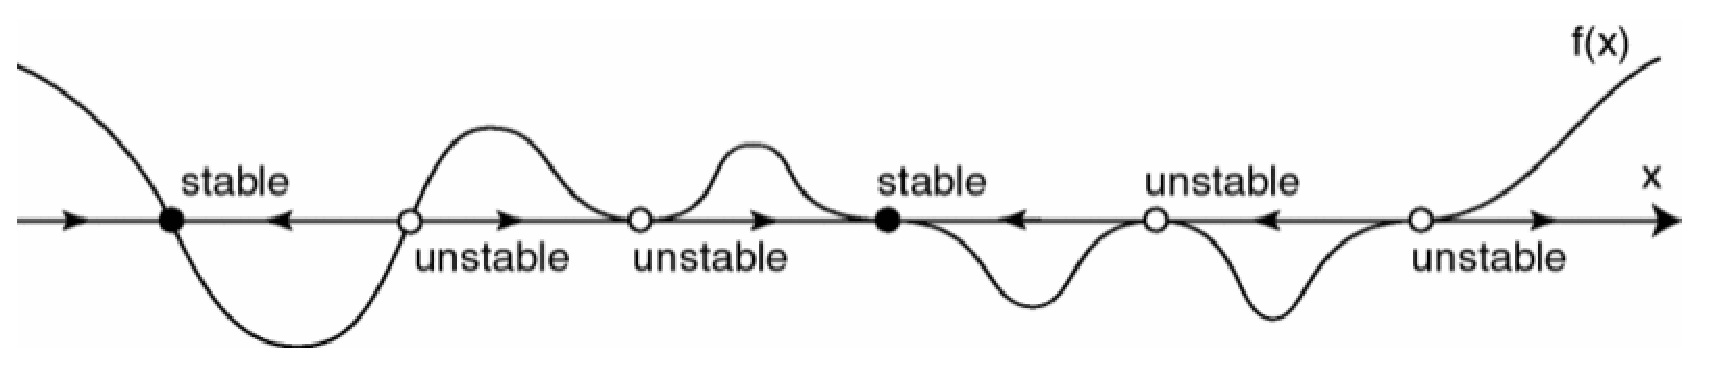
\includegraphics[height=2cm,
    angle=0]{./images/1D_system.eps}}
\caption{1D system with manifold $x_e=0$ (6 times) }
\label{fig:1D_system}
\end{figure}

The two first equilibria are hyperbolic stable. The last 4 equilibria
are non-hyperbolic as the slope (eigenvalue) is zero, i.e. the system
is non-hyperbolic.
\textcolor{red}{In 1D system, the non-hyperbolic system is stable when
  $f(x)$ change its side from positive to negative at the
  equilibrium.} In computer programming, we take first-order
derivative of $f(x,\mu)$ in terms of $x$ and see if
\begin{enumerate}
\item $f_X(x_e,\mu)<0$: the fixed-point is stable
\item $f_x(x_e,\mu)>0$: the fixed-point is unstable
\item $f_x(x_e,\mu)=0$: unknown
\end{enumerate}

\subsection{2D system}
\label{sec:2d-system}

For each equilibrium point, the system has 2 eigenvalues.
\begin{equation}
  \label{eq:647}
  D_x = \left(
    \begin{array}{cc}
      \frac{\partial f}{\partial x} &      \frac{\partial f}{\partial
        y} \\
      \frac{\partial g}{\partial x} &      \frac{\partial g}{\partial
        y} \\
    \end{array}
    \right)
\end{equation}
the eigenvalues can be both real ($a,b$) or complex-conjugate ($a+bi,
a-bi$) (NOTE: a, b:real).
The equilibrium point is then being classified into
\begin{enumerate}
\item {\bf node}: when both eigenvalues are real or of the same sign
\item {\bf saddle}: when both eigenvalues are real or of opposite sign
\item {\bf focus} (spiral-point): when eigenvalues are
  complex-conjugate. the focus are 
  \begin{itemize}
  \item stable when they have negative real part
  \item unstable when they have positive real part
  \end{itemize}
\end{enumerate}

\begin{verbatim}
                 I
                 |
                 |
----------------------------------R
                 |
                 |
\end{verbatim}
Instead of finding eigenvalues, we can classify based on trace $\tau$
and determinant $\Delta$, Fig.~\ref{fig:2D_system}
\begin{equation}
  \label{eq:648}
  \begin{split}
    \tau = \frac{\partial f}{\partial x} + \frac{\partial g}{\partial
      y} \\
    \Delta = \det J
  \end{split}
\end{equation}
\begin{figure}[hbt]
  \centerline{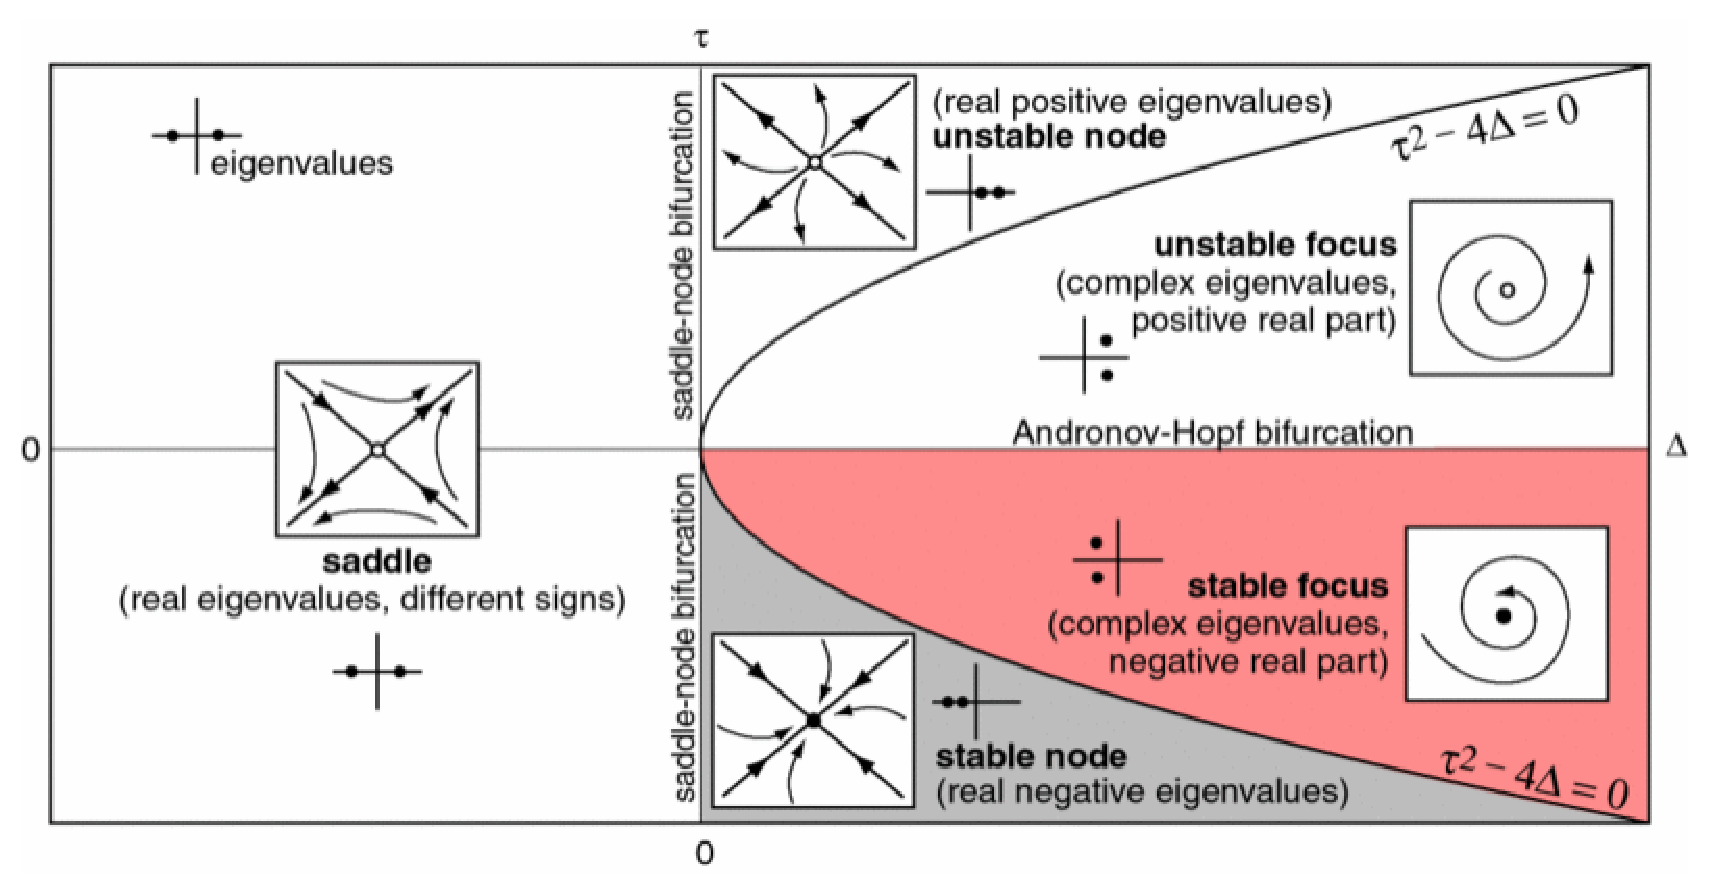
\includegraphics[height=5cm,
    angle=0]{./images/2D_system.eps}}
  \caption{Classification of equilibria according to trace ($\tau$)
    and determinant ($\Delta$)}
\label{fig:2D_system}
\end{figure}
\begin{itemize}
\item The half-axis  $\Delta > 0, \tau=0$ correspond to Andronov-Hopf
  bifurcation 
\item The axis $\Delta =0$ corresponds to saddle-node bifurcation
\end{itemize}

\subsection{3D system}
\label{sec:3d-system}

read \url{http://www.scholarpedia.org/article/Equilibria}




\section{Limit cycle}
\label{sec:limit-cycle}

\subsection{closed trajectory}
\label{sec:closed-trajectory}

In van der Pol oscillation system (Sect.\ref{sec:van-der-Pol-equation}), as
shown in Fig.~\ref{fig:van_der_Pol}, when $\mu=0$, we observe a {\bf closed
trajectory}. It represents a system which can return to its initial state and
has a periodic behavior. However, this is not an interest property of a
non-linear system. What's important is the so-called {\bf limit cycle}.

{\bf NOTE}: Linear-system also has closed trajectory, but they are not
isolated. 

There are situation when the closed trajectory is unstable,
i.e. starting from a point closed to the closed trajectory, the system
will evolve far from this closed trajectory,
Fig.~\ref{fig:limit_cycle_3}(B). There are also system whose behavior
is {\bf half-stable} limit cycle,
Fig.~\ref{fig:limit_cycle_3}(C). 

By default,
\textcolor{red}{limit cycle (Sect.\ref{sec:limit-cycle}) refer to isolated
stable closed trajectory}. The others cases are called unstable closed trajectory
and half-stable closed trajectory.

\subsection{limit cycle}

A limit cycle is a closed trajectory (Sect.\ref{sec:closed-trajectory}) with a
couple of hypothesis: (1) isolated (no other nearby), (2) stable. 

It means that another trajectory must start from somewhere else will approach
this closed trajectory, but never intersect with it, as shown in
Fig.~\ref{fig:limit_cycle}.

\begin{itemize}
\item If it start from a point outside of the closed trajectory, then
  the trajectory become smaller and go closer and closer to the closed
  trajectory.

\item If it start from a point inside of the closed trajectory, then
  the trajectory become bigger and go closer and closer to the closed
  trajectory, but never get out of it.
\end{itemize}


\begin{figure}[hbt]
  \centerline{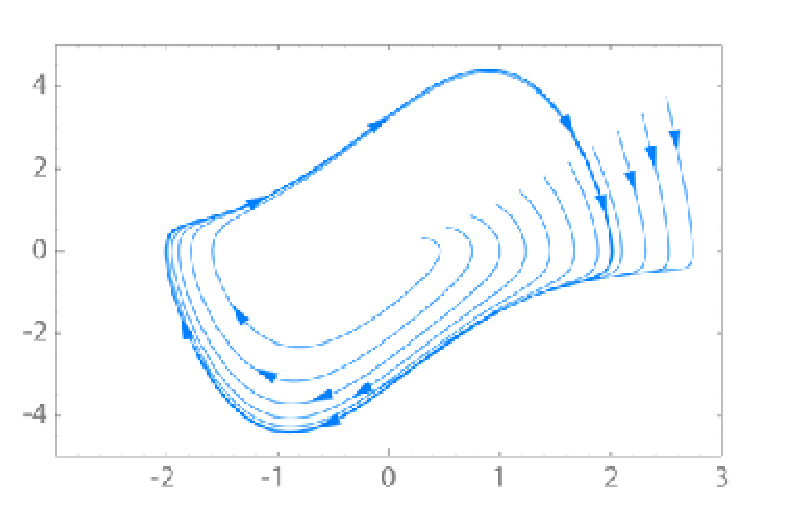
\includegraphics[height=5cm,
    angle=0]{./images/limit_cycle.eps}}
  \caption{Limit cycle}
  \label{fig:limit_cycle}
\end{figure}

In other words,
\textcolor{red}{a limit cycle refer to the property of a non-linear
  system that after a certain amount of time, it reaches the same
  state regardless of the initial condition is}, as shown in
  Fig.~\ref{fig:limit_cycle}.


\begin{figure}[hbt]
  \centerline{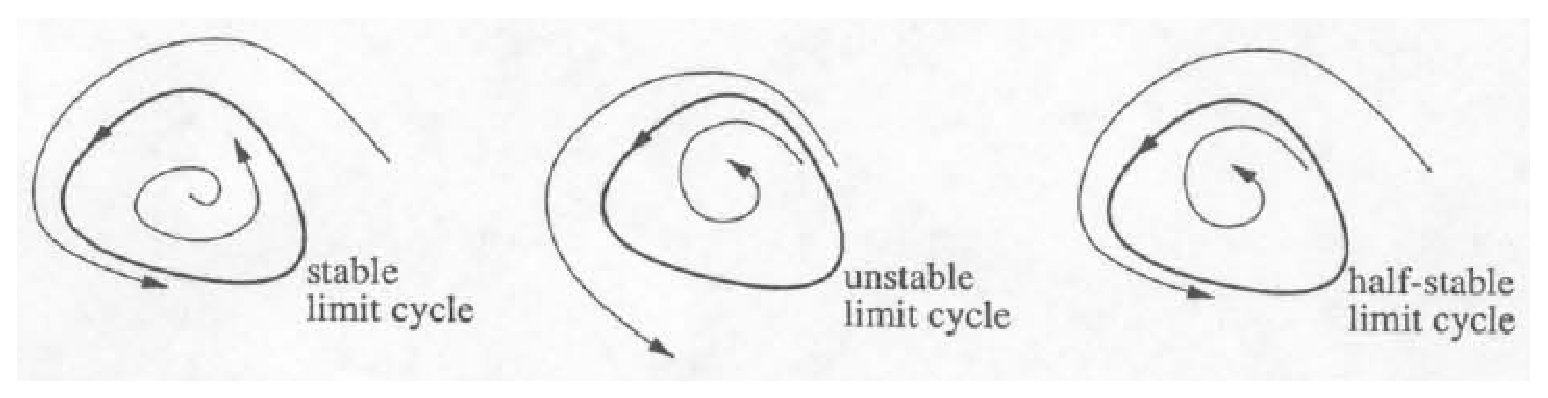
\includegraphics[height=3cm,
    angle=0]{./images/limit_cycle_3.eps}}
  \caption{Limit cycle: stable, unstable and half-stable}
  \label{fig:limit_cycle_3}
\end{figure}

A limit cycle system is called {\it self-sustained oscillator}. Many
systems in nature has limit cycle property, e.g. heart beats,
chemical oscillation, vibration of bridges... If you disturb it,
normally, it will return to its normal behavior after that. Thus, if
the system is modeled correctly, the initial condition of a simulation
is not important, as long as the simulation is long enough, then it
will reach a stable limit cycle. It means that it doesn't depend on
the initial conditions, only the structure of the system.

\subsection{-- detect limit cycle}

There are certain condition to recognize whether a closed trajectory
can be a limit cycle or not:

\begin{enumerate}
\item it must be a simple curve, i.e. it cannot cross itself.
\end{enumerate}

Mathematically (i.e. analytically), we can detect the limit cycle using
Pointcar\'ee-Bendixon theorem. However, nowadays, we mainly use
computer. In certain cases, instead of looking for the limit cycle, we
only need to know the non-existence of the limit cycle, e.g. prove no
closed trajectory. No need to use computer search, maths provides 2
tools: (1) Bendixon - Sect.\ref{sec:bendixon-method}, (2) critical points
(Sect.\ref{sec:crit-point-crit}.


\subsection{---- Bendixon method}
\label{sec:bendixon-method}

We define a region D in plane, then we detect the divergence of the
velocity field $\overrightarrow{\mathbf{F}}$.
\begin{equation}
  \label{eq:584}
  \text{div}\overrightarrow{\mathbf{F}} = f_x + g_y
\end{equation}
if div$\overrightarrow{\mathbf{F}} \ne 0$ at any point in D, then
there is no closed trajectory in D.

{\bf Example}:
\begin{equation}
  \label{eq:585}
  \left\{
    \begin{array}{cc}
      \frac{dx}{dt} = x^3 + y^3\\
      \frac{dy}{dt} = 3x+y^3 + 2y
    \end{array}
  \right.
\end{equation}
then $\text{div}\overrightarrow{\mathbf{F}} = 3x^2+3y^2+2 >
0$. 

To prove this theorem, we can use the indirect method. {\bf Proof}:
Using the previous example, suppose that there exists a closed
trajectory C. Then the flux of $\overrightarrow{\mathbf{F}}$ across C
is defined as
\begin{equation}
  \label{eq:586}
  M = \int_C \overrightarrow{\mathbf{F}}\dot \hat{n} ds
\end{equation}
with $ds$ is the unit length, $n$ is the unit vector pointing outward
straight from the segment of length $ds$ on the surface C, as
$\overrightarrow{\mathbf{F}}$ is the velocity vector perpendicular to
the unit vector at that point, we always have
$\overrightarrow{\mathbf{F}}\cdot \overrightarrow{n}=0$, as a matter of
fact, the above integral is zero.

Now, we apply the Green theorem, which convert the line integral
around a simple curve C to the double integral over the plain region D
bounded by C.
\begin{equation}
  \label{eq:587}
  M =  \int\int_D \text{div}\overrightarrow{\mathbf{F}}dxdy =  \int\int_D \text{div}\overrightarrow{\mathbf{F}}dA
\end{equation}
with $dA = dxdy$ is the unit area. 

Now, given that $\text{div}\overrightarrow{\mathbf{F}} \ne 0$, then it
has to be either 
\begin{itemize}
\item $\text{div}\overrightarrow{\mathbf{F}} > 0$
\item $\text{div}\overrightarrow{\mathbf{F}} < 0$
\end{itemize}
for every point in D. The reason is that if there exist two point with
opposite sign, then based on the continuity property of the function,
there must be exist a point, on the segment connecting these two
points, that receive the value 0. As this point is inside the simple
closed trajectory, it violates the assumption. 

In any case, as a result, the double integral must be either positive
or negative, which violate with eq.~\eqref{eq:586} that get value
zero. Finally, there must not exist a closed trajectory. The Bendixon
is proved. 

Now, we look at another example:
\begin{equation}
  \label{eq:588}
  \left\{
    \begin{array}{cc}
      \frac{dx}{dt} = x^2 + y^2 + 1\\
      \frac{dy}{dt} = x^2-y^2
    \end{array}
  \right.
\end{equation}
Then $\text{div}\overrightarrow{\mathbf{F}} = 2x - 2y$, the values of
(x,y) that cause the divergence zero is the line across the
origin. All points above this line is positive and all points below
this line is negative. So, there is no closed trajectory in either
half of the plane. However, we're not sure if there is/is not a closed
trajectory that across the border line, as shown in
Fig.~\ref{fig:limit_cycle_4}.

\begin{figure}[hbt]
  \centerline{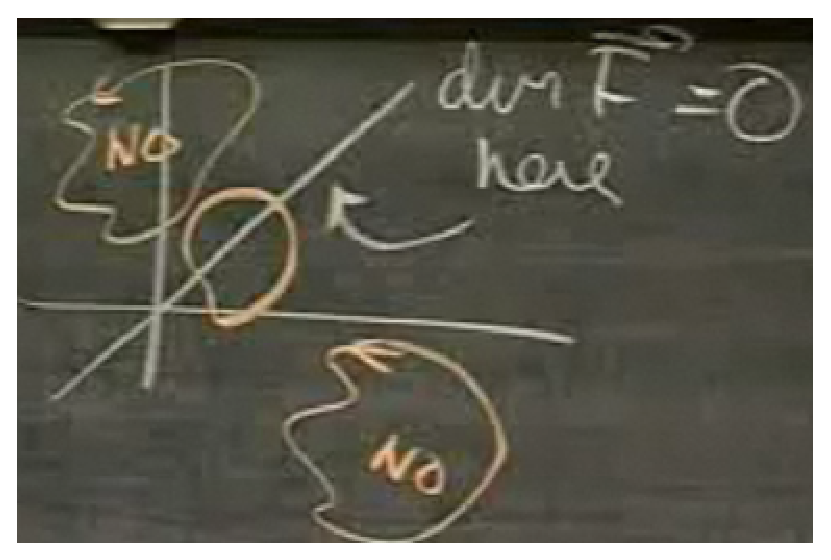
\includegraphics[height=4cm,
    angle=0]{./images/limit_cycle_4.eps}}
  \caption{Limit cycle}
  \label{fig:limit_cycle_4}
\end{figure}

This can be resolved if we use the critical point criterion. 

\subsection{---- Critical point criterion}
\label{sec:crit-point-crit}

We can use critical point criterion to find the existence of a closed
trajectory.
\textcolor{red}{In a region D, i.e. 2-dimension, if it has a closed
  trajectory C, then there must exist a critical point inside C}.
So, the critical point criterion says that:
{\it if there is no critical point inside the region D, there doesn't
  exist any closed trajectory in D}.

In mathematics, a critical point is a point at which the function is
(1) not differentiable or (2) its derivatives is zero. Now, look back
the previous example: $\dot{x} > 0$, then there is no critical
point. We conclude there is no closed trajectory in R, or no limit
cycle. 

\subsection{Summary}
\label{sec:summary-3}


Given a nonlinear system, we may want to
know\footnote{\url{http://www.facstaff.bucknell.edu/mastascu/eControlHTML/Nonlinear/NonLinear1PhasePlane.htm}}

\begin{enumerate}

\item Linear systems might oscillate at a particular frequency, but
  oscillation at a particular amplitude is a phenomenon peculiar to
  nonlinear systems.  That phenomenon is called a limit cycle.

\item Nonlinear systems can exhibit instability when certain inputs
  are applied but may be well behaved (stable) for other inputs.

\item There are very few analytical techniques that can be used to
  predict behavior of nonlinear systems.

  \begin{enumerate}
  \item For comparison, many universities teach courses in Linear
    Systems, and in those courses general techniques for analysis of
    linear systems are taught.
  \item General techniques for analysis of nonlinear systems are hard
    or impossible to find and we are often left to use very specific
    techniques for special situations and we are not able to make
    general statements.

  \end{enumerate}

\item To make predictions of nonlinear system behavior designers often
  use simulations.  However, doing a simulation of a nonlinear system
  only tells the designer about that situation.  There could be other
  situations in which the system misbehaves, and the designer will
  only find that out if s/he does a simulation for that specific
  situation.

\end{enumerate}


References:
\begin{itemize}
\item Theory of Limit Cycles By Yan-Qian Ye, Chi Y. Lo.
\end{itemize}

\section{Centre manifold}
\label{sec:centre-manifold}

This is the central to the development of bifurcation theory. The
reason is that dimension reduction is important to the analysis of a
dynamical system, and centre manifold make this possible, at least
near equilibrium points.

When a system loose the stability, the number of eigenvalues or
eigenvectors associated with this change is normally small. 
Consider a system
\begin{equation}
  \label{eq:650}
  \begin{split}
    \dot{x} = ax^3+xy - xy^2 \\
    \dot{y} = -y + bx + x^y
  \end{split}
\end{equation}
A general form of the system is
\begin{equation}
  \label{eq:651}
  \begin{split}
    \dot{x} = Ax + f(x,y) \\
    \dot{y} = By + g(x,y)
  \end{split}
\end{equation}
with $x\in \mathbb{R}^n, y\in \mathbb{R}^m$.  The two function are
smooth (C$^\infty$) function 



\section{Linear stability vs. nonlinear stability}
\label{sec:linear-stability-vs}

Here, we discuss the relation between linear stability vs. nonlinear
stability w.r.t small disturbance. 


\section{Bifurcation in 1D}
\label{sec:bifurcation-1d}

The phase plane analysis plot $\dot{X}$ vs. $X$. 
\subsection{Saddle-node bifurcation}
\label{sec:saddle-node-bifurc}
%\section{Saddle-node bifurcation}
\label{sec:bifurcation-saddle-node}

Fig.\ref{fig:bifurcations}, the V$_\text{PLC}$ values required for oscillations
are considerably smaller in the negative-feedback model than in the
positive-feedback model..

This bifurcation occur when
\textcolor{red}{there is a creation or destruction of
  fixed-points}. The basic example is
\begin{equation}
  \label{eq:668}
  \dot{x} = \mu + x^2
\end{equation}
with $\mu$ is the controlling parameter.

To find the fixed-point (FP), we set $\dot{x}=0$, i.e. solve the equation
\begin{equation}
  \label{eq:56}
  x^2 + \mu = 0
\end{equation}
So, the number of FP depends on $\mu$.
\begin{itemize}
\item $\mu < 0$: two FPs
\item $\mu = 0$: one FP
\item $\mu > 0$: no FP
\end{itemize}
we draw $f(x,\mu)=x^2+\mu$ on $x$ vs. $\dot{x}$ coordinate. Find the
intersection when $f(\cdot) = 0$, combining with vector field, we can
tell which FP is stable and unstable, Fig.~\ref{fig:saddle_node_ex1}.

\begin{figure}[hbt]
  \centerline{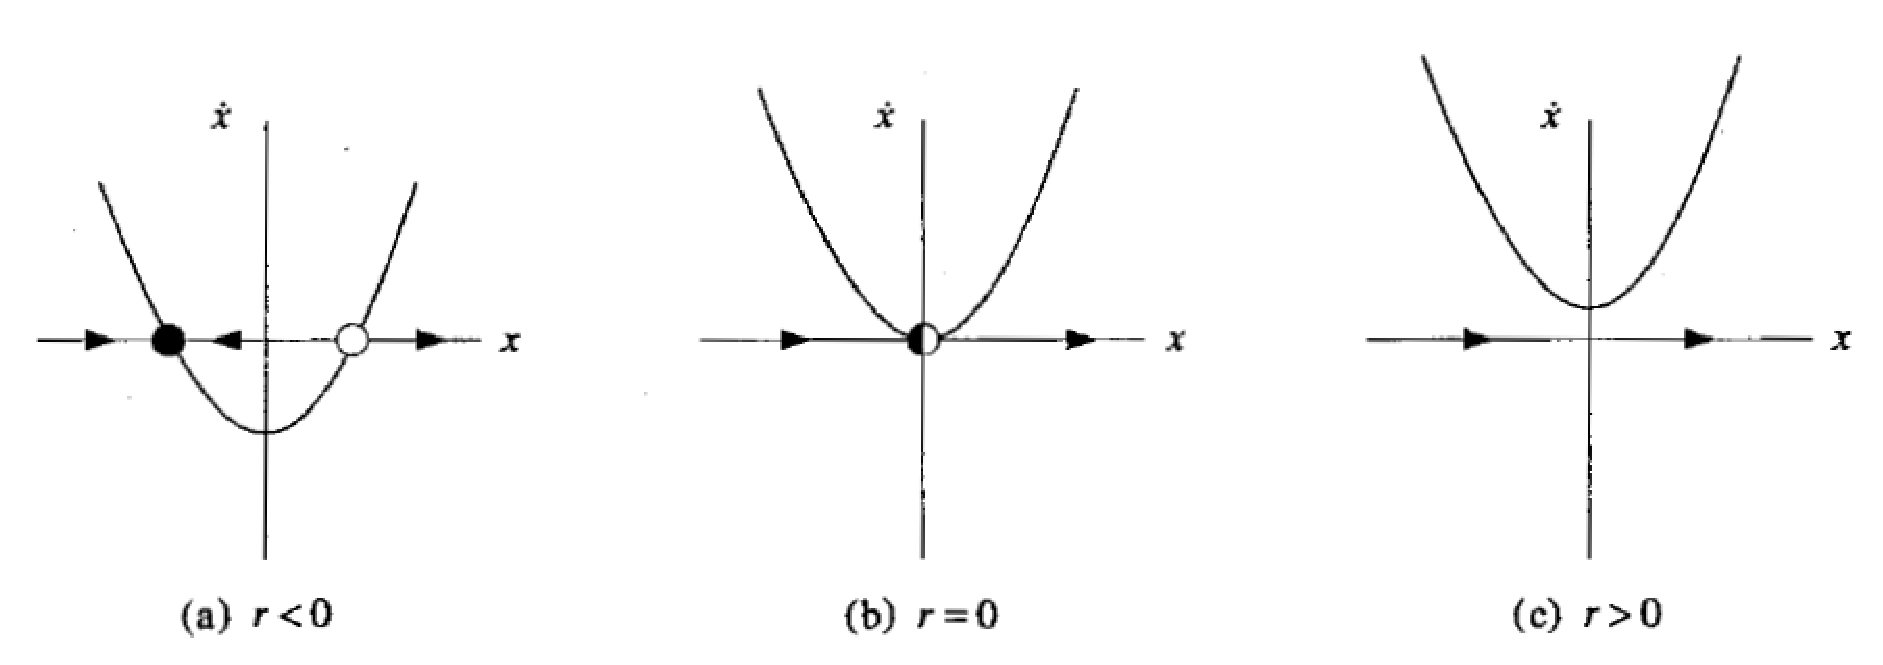
\includegraphics[height=5cm,
    angle=0]{./images/saddle_node_ex1.eps}}
\caption{filled circle: stable FP, white circle: unstable FP, the
  arrow tell the trend of the change of the system}
\label{fig:saddle_node_ex1}
\end{figure}

{\bf NOTE}: Both $\dot{x}=\mu - x^2$ and $\dot{x}=\mu + x^2$  are
representative of saddle-node bifurcation. The idea is that close to a
saddle-node bifurcation, the dynamics typically look like one of the
two equations. These equations are known as {\bf normal form} or
prototypical form. 

\textcolor{red}{How to draw the bifurcation?}
  Fig.~\ref{fig:saddle_node_bifur}: Draw the coordinate $x$ vs. $\mu$
  ($\mu$ on the horizontal axis). Draw the nullclines for
  eq.~\eqref{eq:668}. Here it is
\begin{equation}
  \label{eq:681}
  x = \pm \sqrt{-\mu}; \text{ with } \mu < 0
\end{equation}
Looking at Fig.~\ref{fig:saddle_node_ex1}, the stable node is the one
when $x<0$, then we keep the lower part as solid, the upper part as
dotted.
\begin{figure}[hbt]
  \centerline{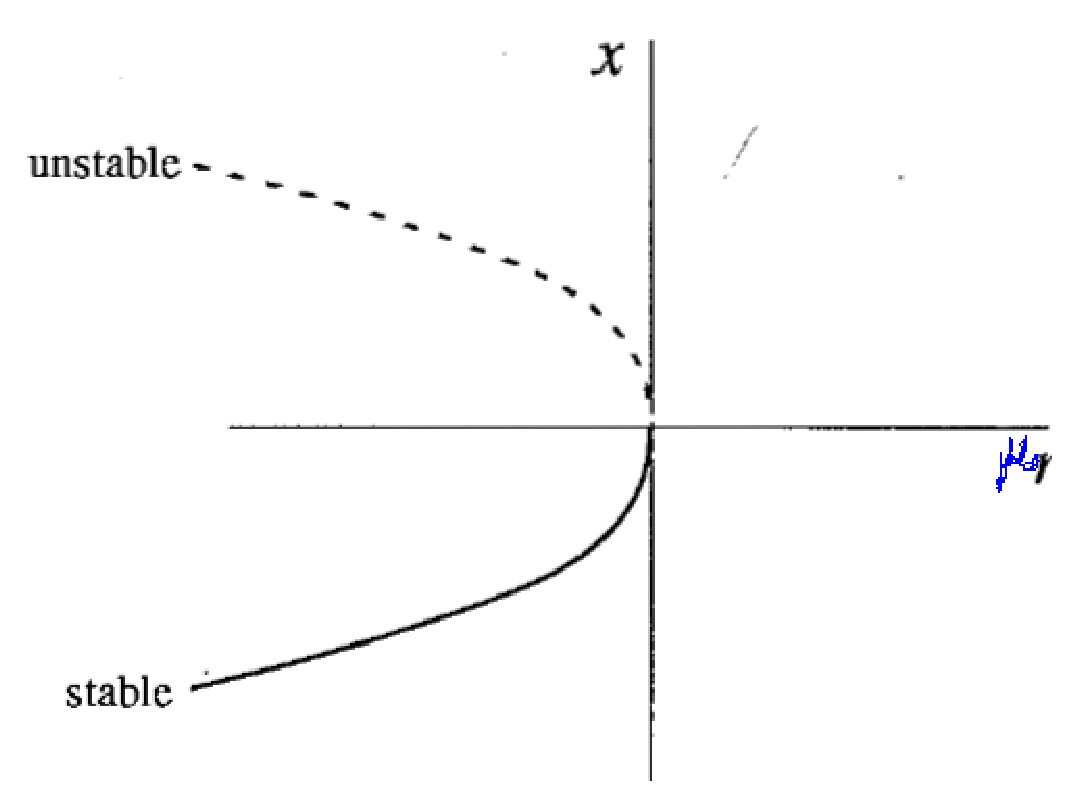
\includegraphics[height=5cm,
    angle=0]{./images/saddle_node_bifur.eps}}
  \caption{solid line = set of stable FP when changing control
    parameter $\mu$; dotted line = set of unstable FP}
  \label{fig:saddle_node_bifur}
\end{figure}

Example:
\begin{equation}
  \label{eq:103}
  \dot{x} = \mu - x - e^{-x}
\end{equation}
has a saddle-node bifurcation. This can be proved by mapping to the
above prototypical form. Here, we use Taylor expansion
\begin{equation}
  \label{eq:679}
  \begin{split}
    \dot{x} = \mu - x - \left[1 - x + \frac{x^2}{2} ...\right] \\
    &= (\mu - 1) - \frac{x^2}/2 + ...
  \end{split}
\end{equation}
We just keep at the second-order of the expansion. If we define
$x=x/\sqrt{2}$, then
\begin{equation}
  \label{eq:680}
  \dot{x} = k - x^2
\end{equation}
with $k=(\mu-1)$. 


\subsection{Transcritical bifurcation}
\label{sec:transcr-bifurc}

There are situation when a fixed-point must always be exist for all
values of the parameter and can never be destroyed. However, the
stability of the system at that FP may change.  
\begin{equation}
  \label{eq:670}
  \dot{x} = \mu x - x^2
\end{equation}
The minus can be plus, it's not important. When $\mu$ change the side,
there is the switch of stability between the two FPs. The important
note is that, after the bifurcation, the two FPs doesn't disappear,
they just switch the stabilities, Fig.~\ref{fig:transcritical}.

\begin{figure}[hbt]
  \centerline{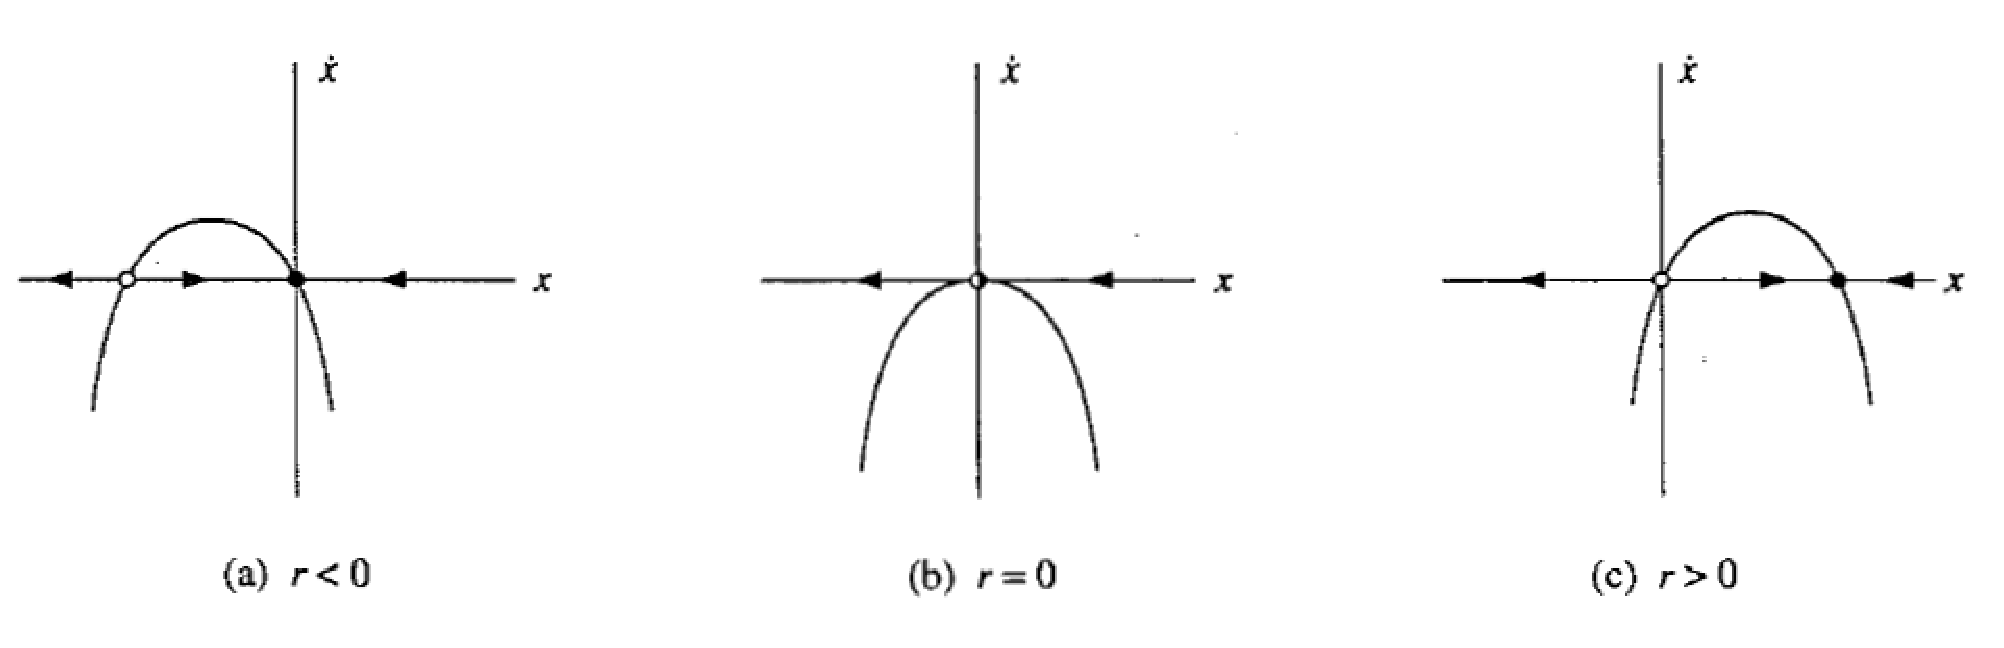
\includegraphics[height=4cm,
    angle=0]{./images/transcritical_ex1.eps}}
\caption{nullcline}
\label{fig:transcritical}
\end{figure}

\textcolor{red}{How to draw the bifurcation?} Fig. We draw the
coordinate $x$ vs. $\mu$ ($\mu$ on the horizontal axis). Draw the
nullclines for eq.~\eqref{eq:670}. Here it is
\begin{equation}
  \label{eq:682}
  \begin{split}
    \left [
      \begin{array}{c}
        x = 0 \\
        x = \mu
      \end{array}
      \right.
  \end{split}
\end{equation}
Looking at the phase plane, for the first line, the system is stable
only when $\mu < 0$. For the second line $x=\mu$ stable only when
$\mu>0$, Fig.~\ref{fig:transcritical_bifur}.
\begin{figure}[hbt]
  \centerline{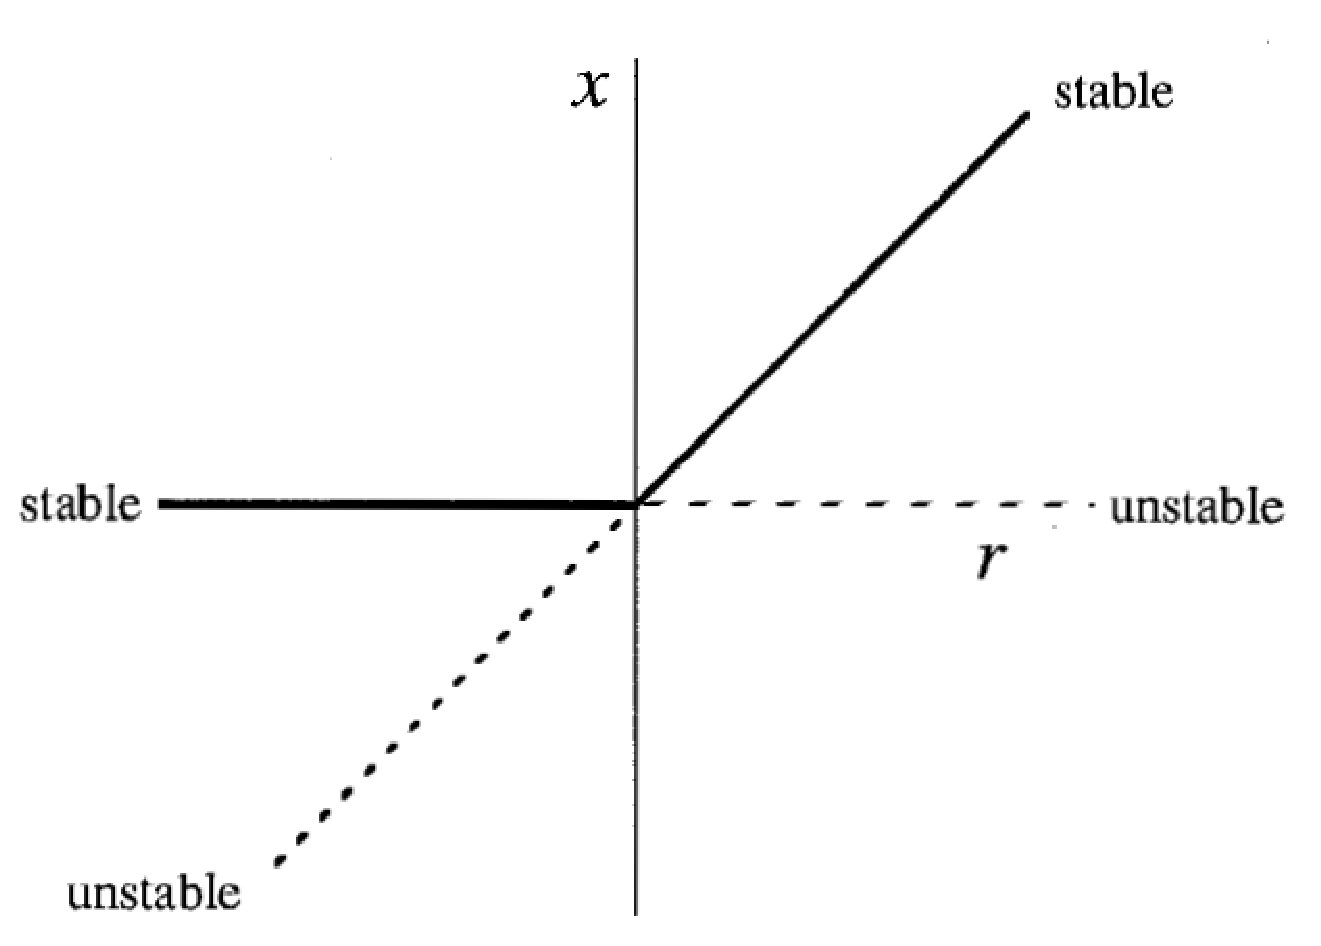
\includegraphics[height=5cm,
    angle=0]{./images/transcritical_bifur.eps}}
\caption{Transcritical bifurcation}
\label{fig:transcritical_bifur}
\end{figure}

In practice, transcritical systems rarely exist such system. 

\subsection{Pitchkorf bifurcation}
\label{sec:pitchk-bifurc}

For the system to be symmetric, the first-order ODE must be of higher
than or equal 3.

There are two cases:

\subsubsection{supercritical pitchfork bifurcation}
\label{sec:supercr-pitchf-bifur}

\begin{equation}
  \label{eq:671}
  \dot{x} = \mu x - x^3
\end{equation}
The system is called {\bf invariant} as when we substitute $x$ by
$-x$, the system doesn't change.

The decay, if exponential, is considered fast. However, consider
$\dot{x}=-x^3$, then $x(t+1)=x(t)-dt*x(t)^3$ the decay is ``critical
slowing down'' (due to second-order phase transition). Now look at
$\dot{x}=-x$, then $x(t+1)=x(t)-dt*x(t)$. As $x$ is close to zero,
$x^3$ change slower than $x$. 

\begin{figure}[hbt]
  \centerline{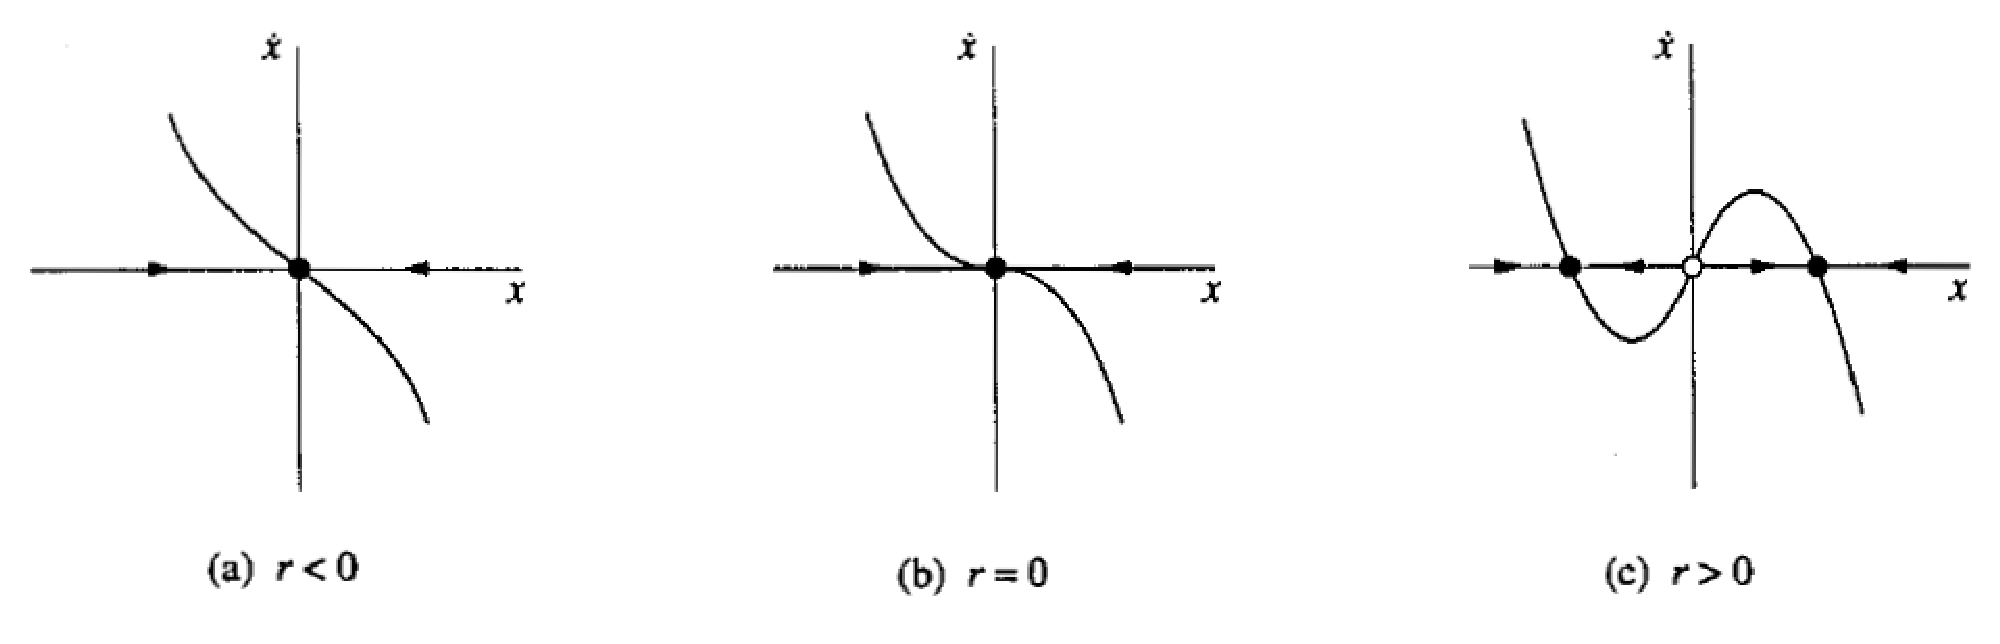
\includegraphics[height=5cm,
    angle=0]{./images/pitchfork_ex1.eps}}
\caption{}
\label{fig:pitchfork_ex1}
\end{figure}

\textcolor{red}{How to draw the bifurcation?} Fig. We draw the
coordinate $x$ vs. $\mu$ ($\mu$ is the horizontal axis). Detect the
always-there FP $x=0$ (when $\mu<0$). When $\mu>0$, we have another
curve $\mu=x^2$, all $x$ in here are stable. At the same time, the old
FP $x=0$ become saddle. However, the variation in the system is not
big, but smoothly when $\mu$ go to positive size.

\begin{figure}[hbt]
  \centerline{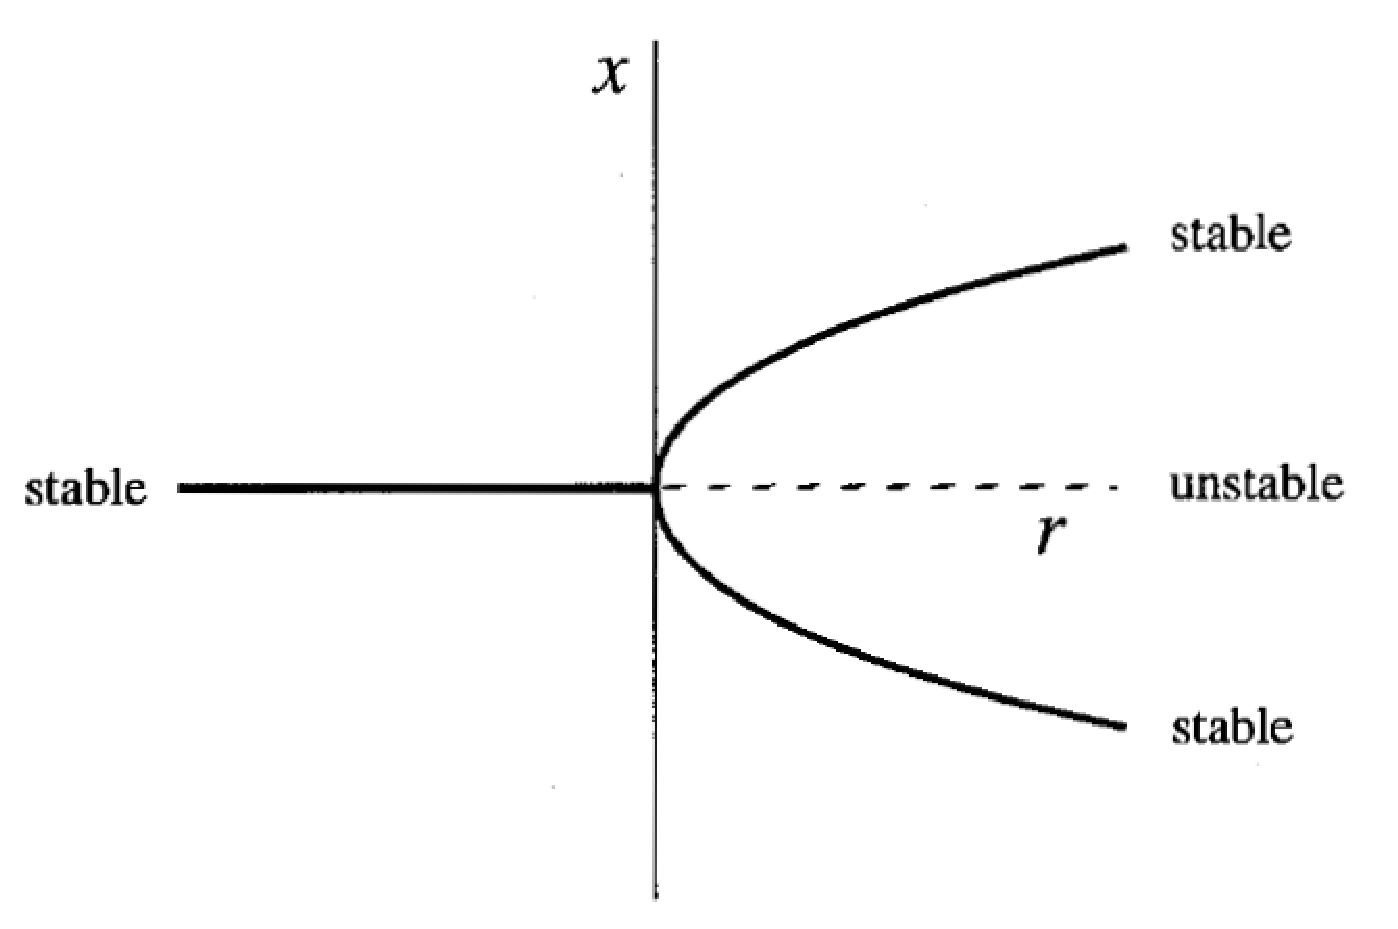
\includegraphics[height=5cm,
    angle=0]{./images/pitchfork_bifur.eps}}
\caption{Supercritical Pitchfork bifurcation}
\label{fig:pitchfork_bifur_super}
\end{figure}


\subsubsection{subcritical pitchfork bifurcation}
\label{sec:subcr-pitchf-bifurc}

\begin{equation}
  \label{eq:672}
  \dot{x} = \mu x + x^3
\end{equation}


\section{Bifurcation in 2D}
\label{sec:bifurcation-2d}

From 2D, we will have Hopf bifurcation. In 2D, we'll have the
appearance/disappearance of closed orbit. However, we still observe
the appearance and disappearance of fixed-points. So, Saddle-node
bifurcation will be discussed also. 

In 1D, when we study the topological change in a system, we study the
change when the parameter cause the system vary a little bit from the
fixed-point. So, before running bifurcation analysis, the system need
to reach the fixed-point. That's why we'll need to run the simulation
a while until the system reach the steady-state value
(\textcolor{blue}{XPP (Sect.\ref{sec:xpp-tool}): I-G (I-L)$^n$ with $n$ is a
number of time to press I-L}).

The topological change or we say ``a bifurcation occur'' involves
change in the number of stability of
\begin{enumerate}
\item fixed-points
\item closed orbits
\item saddle connection
\item ...
\end{enumerate}


\section{Homoclinic bifurcation}
\label{sec:bifurcation-homoclinic}

Fig.\ref{fig:bifurcations}, a homoclinic bifurcation is associated with the
existence of multiple steady states, which arise through saddle-node
bifurcations (Sect.\ref{sec:bifurcation-saddle-node}).

In the given example, such multistationarity is typical for models that neglect
the plasmamembrane fluxes of calcium.



\begin{figure}[hbt]
  \centerline{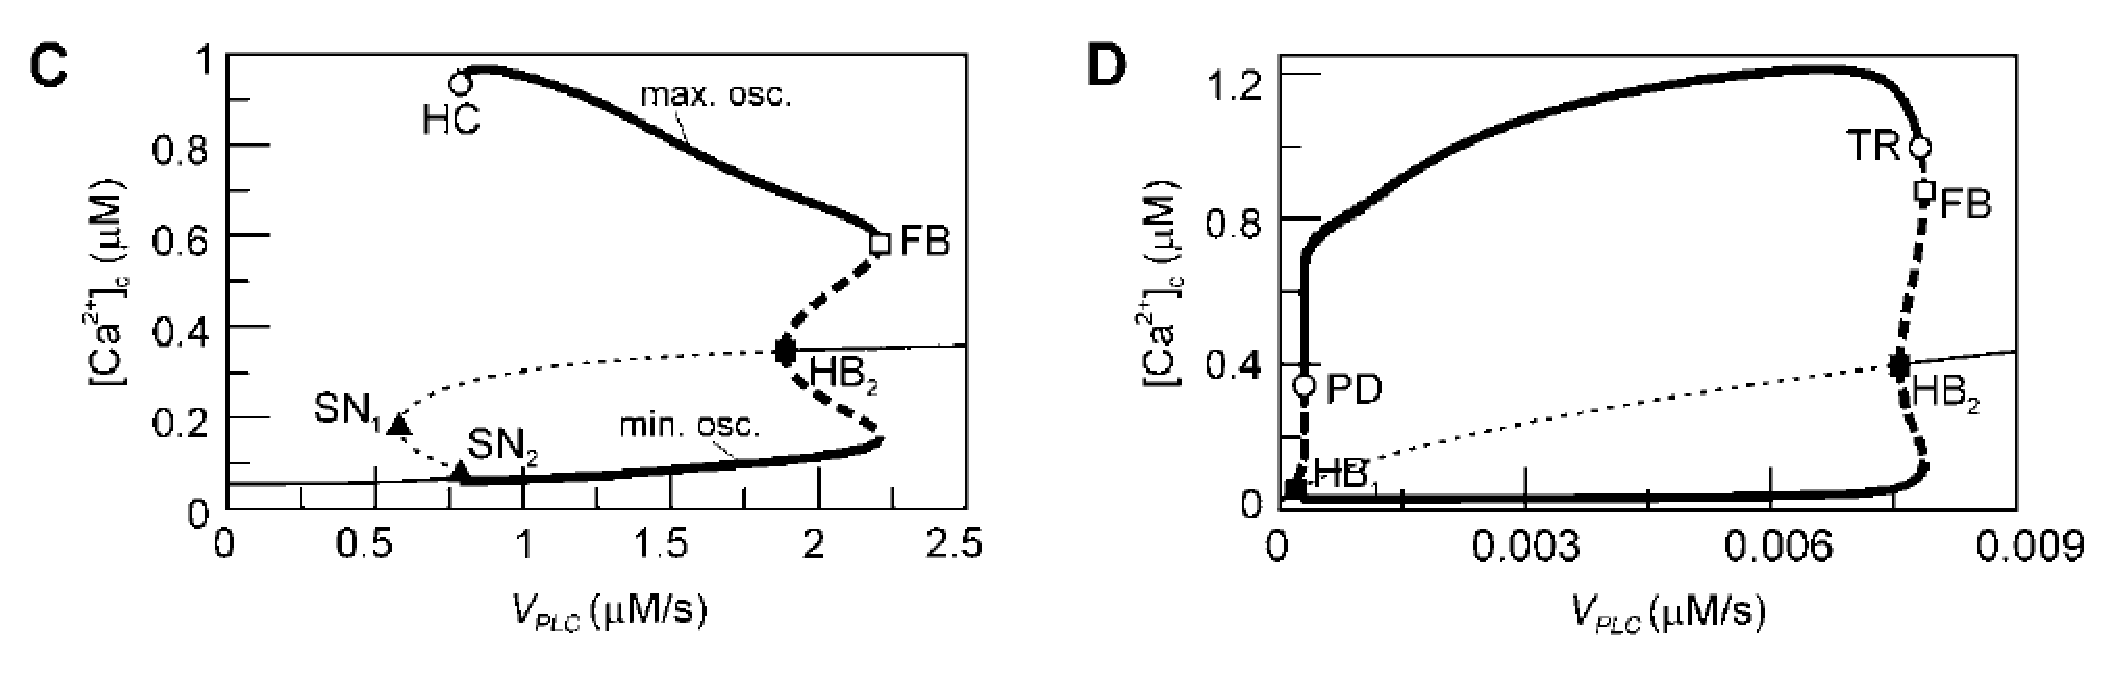
\includegraphics[height=5cm,
    angle=0]{./images/bifurcations.eps}}
\caption{Solid and dashed lines indicate stable and unstable states. (C)
Bifurcation diagram for positive feedback model. Bifircations: HB, Hopf bifurcation; HC, homoclinic bifurcation; SN,
saddle-node bifurcation; FB, saddle node of periodics. (D) Bifurcation diagram for negative
feedback model. PD, period doubling; TR, torus bifurcation. Between PD and HB1
and TR and FB there exist complex oscillations (omitted for clarity). 
\textcolor{red}{thick lines} = maxima and minima of calcium oscillations;
\textcolor{red}{thin lines} = steady-state values of calcium as the function of
the stimulus v$_\text{PLC}$ }
\label{fig:bifurcations}
\end{figure}

\section{Torus bifurcation}
\label{sec:bifurcation-torus}

Fig.\ref{fig:bifurcations}


\section{Hopf bifurcation}
\label{sec:hopf-bifurcation}
\label{sec:bifurcation-Hopf}

Hopf bifurcation is the bifurcation occur when the system is 2D, and
when it is disturbed from the fixed-point, along with the formation of
a closed periodic orbit around the equilibrium point, as shown in
Fig.~\ref{fig:Hopf_bifurcation}.

\begin{figure}[hbt]
  \centerline{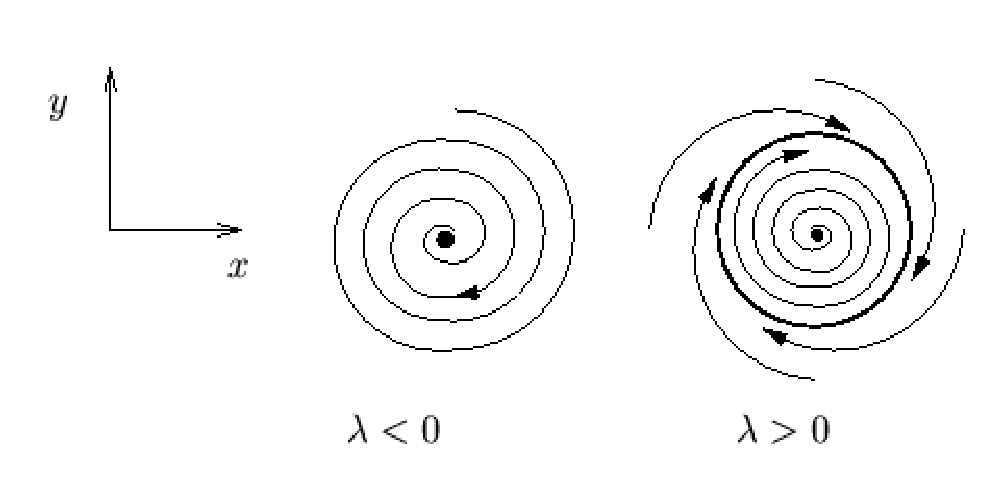
\includegraphics[height=5cm,
    angle=0]{./images/Hopf_bifurcation.eps}}
\caption{$\lambda<0$: stable fixed point, $\lambda>0$ the unstable
  fixedpoint and a stable periodic orbit}
\label{fig:Hopf_bifurcation}
\end{figure}

In the negative-feedback model, Fig.\ref{fig:bifurcations}(D), there are two
regions near the Hopf bifurcations HB1 and HB2 (before the point PD and after
the point TR) where irregular and bursting oscillations are observed.
Because these two regions are extremely narrow, compared to the total
stimulation range in the negative feedback model, our focus will be on the
regular oscillations (Politi et al., 2006).

\subsection{Supercritical Hopf bifurcation}
\label{sec:supercr-hopf-bifurc}


Consider a exponentially damping oscillation, as shown in
Fig.~\ref{fig:exp_damp_osci}. Suppose the decay rate depend on a
control parameter $\mu$. If the decay become slower and slower, then
at a certain point, we call $\mu=\mu_c$ as critical point, we doesn't
have decay any more. If we continue to decrease $\mu$, the decay
become the growth.

\begin{figure}[hbt]
  \centerline{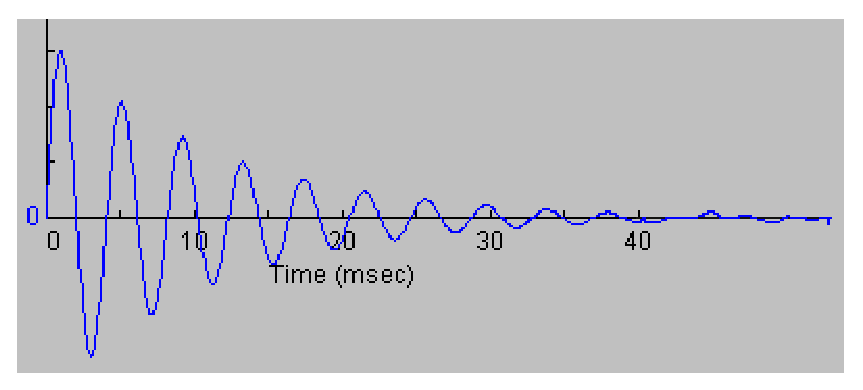
\includegraphics[height=5cm,
    angle=0]{./images/exp_damp_osci.eps}}
\caption{Exponentially damping oscillation}
\label{fig:exp_damp_osci}
\end{figure}

At $\mu=\mu_c$, we have ellipsoidal oscillation. A small change in
$\mu$ only cause a small change in the oscillation, i.e. the small
change in the limit cycle, then we have supercritical Hopf
bifurcation. 

Example:
\begin{equation}
  \label{eq:673}
  \begin{split}
    \dot{r} = \mu r - r^3 \\
    \dot{\theta} = \omega + br^2
  \end{split}
\end{equation}
We can switch back to the Cartesian coordinate using 
\begin{equation}
  \label{eq:674}
  x=r\cos\theta \; ; \; y = r\sin\theta
\end{equation}
or 
\begin{equation}
  \label{eq:676}
  \begin{split}
    \dot{x} = \mu x - \omega y + \text{cubic term} \\
    \dot{y} = \omega x + \mu y + \text{cubic term}
  \end{split}
\end{equation}


Two rules of thumb for supercritical Hopf bifurcation:
\begin{enumerate}
\item From the critical fixed-point (i.e. bifurcation point, and with
  zero limit cycle), it increases continuously, i.e. forming the limit
  cycle, and increase proportional to $\sqrt{\mu-\mu_c}$, for $\mu$
  closed to $\mu_c$.
\item Frequency of the limit cycle is given approximately by
  $\omega=\text{Im}\lambda$, evaluated at $\mu=\mu_c$.
\end{enumerate}
The limit cycle is elliptical, not circular, and its shape become
distorted as $\mu$ moves away from bifurcation point.

\subsection{Subcritical Hopf bifurcation}
\label{sec:subcr-hopf-bifurc}

The subcritical Hopf bifurcation is quite different than supercritical
one. After leaving the bifurcation point, the system abruptly change
the behavior, and jump to a new {\it distant}  attractor, which can be
a fixed-point, a new limit cycle, infinity (go to any where so far) or
(only in 3D and above) chaotic attractor. 

\begin{equation}
  \label{eq:675}
  \begin{split}
    \dot{x} = \mu x + x^3 - x65 \\
    \dot{\theta} = \omega + br^2
  \end{split}
\end{equation}
Here, we also have the cubic term, yet it help destabilizing the
system. This causes the problem to the system. 

When $\mu>0$, solution closed to $\mu_c=0$, now tend to move away and
jump to the limit cycle outside. This limit cycle represent a voltage
oscillation (as we often see in neuronal cells).


{\bf TIPS}: In order to tell if a bifurcation is Hopf bifurcation,
there must be a limit cycle (stable or unstable is not important)
there must be a closed orbit. It cannot be a spiral. This case is
called {\bf degenerate Hopf bifurcation}. 

{\bf TIPS}: To tell if a Hopf bifurcation is supercritical or subcritical, we
need to use computer mainly. Analytical technique is very hard to use. One
common option is using AUTO package (available from XPPAUT -
Sect.\ref{sec:xpp-tool}), we look at the critical fixed-point (the bifurcation
point), if at its proximity, a small, attracting limit cycle appears, and shrink
back to zero if $\mu$ reverse back to the bifurcation point, then it is {\it
  supercritical Hopf bifurcation}. Otherwise, if the system go up or
down far away from that point, it is subcritical Hopf bifurcation.

Example:
\begin{equation}
  \label{eq:677}
  \begin{split}
    \dot{x}  = \mu x - y + xy^2 \\
    \dot{y} = x + \mu y + y^3
  \end{split}
\end{equation}


\section{Bifurcation in 3D}
\label{sec:bifurcation-3d}

In 3D, besides the fixed-point and limit cycle concepts, we also have
the chaotic attractor.

\section{Bifurcation in chemical reaction}
\label{sec:bifurc-chem-react}

It has long been believed that any chemical reaction, at a certain
point in time, must reach equilibrium state, i.e. no change in
concentration of substances. Belousov (1950s) was the first one to try
to create an oscillation chemical reaction. His work was rejected by
all journals that time. There are the so-called {\bf spiral waves} in
chemical reactions.

Spiral waves are now recognized as a ubiquitous feature of chemical,
biological and physical excitable media. Its 3D analogous is {\bf
  scroll waves} appear to be implicated in certain cardiac
arrhythmias. 

\section{Homoclinic bifurcation}
\label{sec:homocl-bifurc}

Homoclinic bifurcation is a kind of {\bf infinite-period}
bifurcation. It's infinite, because it takes forever to pass the
saddle node on the limit. It's also called
{\bf saddle-loop bifurcation}. Its many other names are
\begin{enumerate}
\item saddle-node bifurcation on invariant circle (SNIC) 
\item saddle-node on limit cycle (SNLC)
\end{enumerate}
Here, the center manifold forms a limit cycle. 

\begin{figure}[hbt]
  \centerline{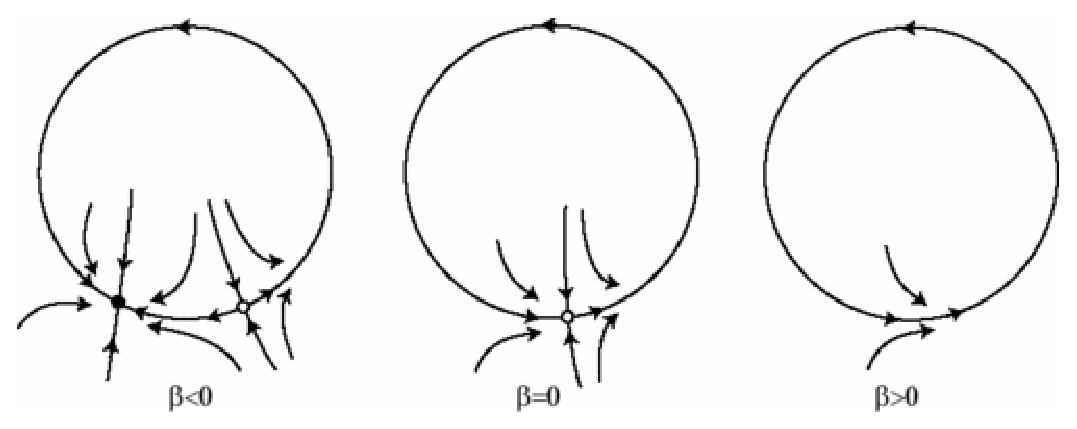
\includegraphics[height=5cm,
    angle=0]{./images/SNIC_bifurcation.eps}}
\caption{SNIC bifurcation}
\label{fig:SNIC}
\end{figure}

\subsection{Eliminate time element}
\label{sec:elim-time-elem}

In many cases, it is enough to use bivariate autonomous system only.
In a 2D autonomous first-order system, geometrically, it is
represented by a {\it vector field} $\overrightarrow{\mathbf{F}}$
\begin{equation}
  \label{eq:582}
  \overrightarrow{\mathbf{F}} = (\dot{x},\dot{y}) 
\end{equation}
The direction of the vector tell the trend of the change of the
system. The length of the vector field will tell us how fast the
system change at that point.

In many cases, to make it easier to study a system, the time element
should be removed.  In 2D system, this can be achieved by dividing one
of these equations by the other

\begin{equation}
  \label{eq:591}
  \frac{dy}{dx} = \frac{f(x,y)}{g(x,y)}
\end{equation}
Here we convert from a non-linear system to a single ordinary
first-order differential equation to which we can apply many methods
to analyze.

However, when we remove the time element, all vector fields are
normalized and we lost the length information. What we have is just
the direction. In other words, instead of the vector field we now have
the {\bf direction field} in which all vectors are normalized to the
same length, as shown in Fig.~\ref{fig:vector_field}.

\begin{figure}[hbt]
  \centerline{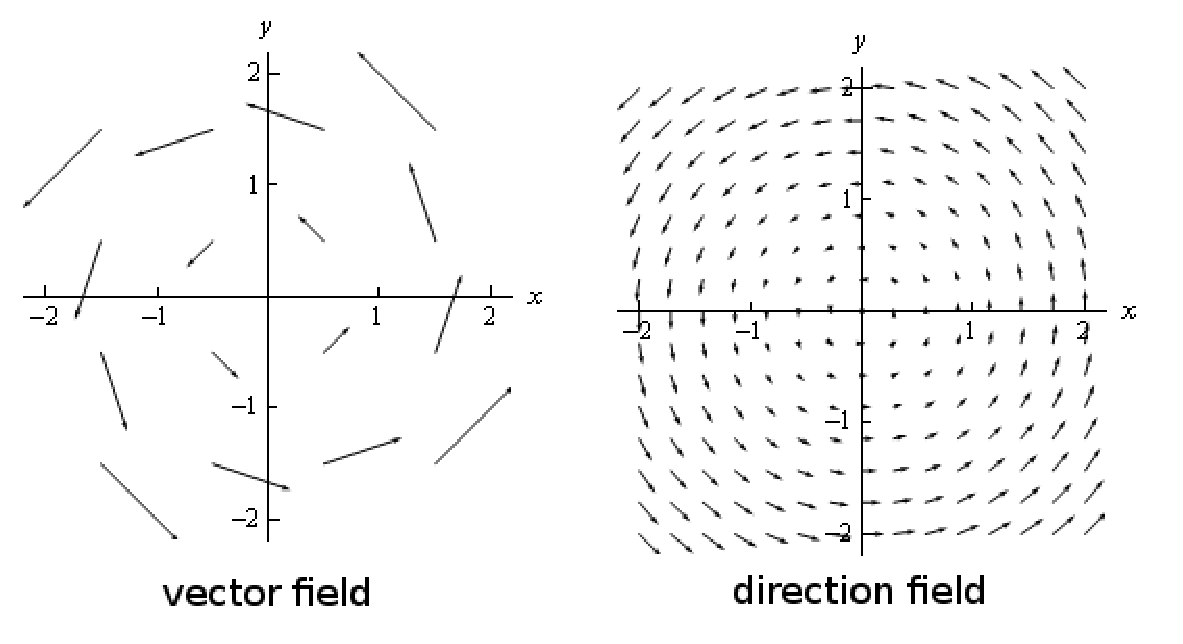
\includegraphics[height=5cm,
    angle=0]{./images/vector_field.eps}}
  \caption{(A) Vector field, (B) Direction field}
  \label{fig:vector_field}
\end{figure}

We don't have the trajectory anymore, instead, it is the
{\bf integral curve}. The question, why we eliminate $t$ when we lost
too many information. The big point is the eq.~\eqref{eq:582} is
almost impossible to solve, while the eq.~\eqref{eq:591} is
solvable. We will discuss in detail in
Sect.~\ref{sec:predator-prey-model}.

\textcolor{red}{Tools to plot vector field/direction field: Maple,
  Mathematica}\footnote{\url{http://tutorial.math.lamar.edu/Classes/CalcIII/VectorFields.aspx}}. 

{\bf Example}:
\begin{equation}
  \label{eq:368}
  \frac{dy}{dx} = -\omega_0^2\frac{x}{y}
\end{equation}


\section{Software tools}
\label{sec:software-tools}


You can use
\begin{enumerate}
\item XPPAUT (still very useful)
\item Phaser
\item MacMath (outdate, for Mac)
\item DynPac package from Mathematica
\end{enumerate}

References:
\begin{enumerate}
\item Nonlinear Dynamics and Chaos - Steven H. Strogatz
\end{enumerate}
% In the previous chapter, in phase plane analysis, we also
% study how the system change when varying

\section{TIPS}
\label{sec:tips}

A signal to tell if a system has saddle-node bifurcation is 
\begin{itemize}
\item the FP can appear disappear when we change $\mu$
\end{itemize}

A signal to tell if a system has transcritical bifurcation is
\begin{itemize}
\item we always have a FP
\end{itemize}

A signal to tell if a system has a pitchfork bifurcation is
\begin{itemize}
\item the system has symmetry, i.e. has oscillation.
\end{itemize}


Many system can be mapped to any of the above normal form using Taylor
expansion
\begin{equation}
  \label{eq:683}
  \begin{split}
    \ln(1+u) = u - \frac{1}{2}u^2 + O(u^3) \\
    e^{-ax} = 1 - ax + \frac{1}{2} (ax)^2 + O(x^3)
  \end{split}
\end{equation}

%%% Local Variables: 
%%% mode: latex
%%% TeX-master: "mainfile"
%%% End: 
